\section{Formulate Statement}

\subsection{ Redefinition of Narrow RevTerminate Principle}
相較於 informal logic proof, we need 更嚴格的定義 for our formal logic proof.
Here is the Narrow RevTerminate Principle:
``Given a reversible abstract machine with a finite number of total states, it will inevitably terminate from any initial state.''

First of all, we define the initial state.  Given a state, if 他不是任何state的next state,we call the state is initial.
\begin{code}%
\>[2]\AgdaFunction{is-initial} %
\AgdaSymbol{:} %
\AgdaField{State} %
\AgdaSymbol{→} %
\AgdaPrimitive{Set} %
\AgdaSymbol{\AgdaUnderscore{}}\<%
\\
%
\>[2]\AgdaFunction{is-initial} %
\AgdaBound{st} %
\AgdaSymbol{=} %
\AgdaFunction{∄[} %
\AgdaBound{st'} %
\AgdaFunction{]} %
\AgdaSymbol{(}\AgdaBound{st'} %
\AgdaOperator{\AgdaField{↦}} %
\AgdaBound{st}\AgdaSymbol{)}\<%
\\
\>[0]\<%
\end{code}

Secondly, we define the terminate of a reversible machine.
Starting from the initial state $st_{0}$, we use $st_{0}$ $\mapsto$* $st_{n}$ presents $st_{0}$ can reach $st_{n}$ by walk through finite steps.
\begin{code}%
    \>[2]\AgdaKeyword{data} %
    \AgdaOperator{\AgdaDatatype{\AgdaUnderscore{}↦*\AgdaUnderscore{}}} %
    \AgdaSymbol{:} %
    \AgdaField{State} %
    \AgdaSymbol{→} %
    \AgdaField{State} %
    \AgdaSymbol{→} %
    \AgdaPrimitive{Set} %
    \AgdaSymbol{(}\AgdaPrimitive{L.suc} %
    \AgdaBound{ℓ}\AgdaSymbol{)} %
    \AgdaKeyword{where}\<%
    \\
    \>[2][@{}l@{\AgdaIndent{0}}]%
    \>[4]\AgdaInductiveConstructor{◾} %
    \AgdaSymbol{:} %
    \AgdaSymbol{\{}\AgdaBound{st} %
    \AgdaSymbol{:} %
    \AgdaField{State}\AgdaSymbol{\}} %
    \AgdaSymbol{→} %
    \AgdaBound{st} %
    \AgdaOperator{\AgdaDatatype{↦*}} %
    \AgdaBound{st}\<%
    \\
    %
    \>[4]\AgdaOperator{\AgdaInductiveConstructor{\AgdaUnderscore{}∷\AgdaUnderscore{}}} %
    \AgdaSymbol{:} %
    \AgdaSymbol{\{}\AgdaBound{st₁} %
    \AgdaBound{st₂} %
    \AgdaBound{st₃} %
    \AgdaSymbol{:} %
    \AgdaField{State}\AgdaSymbol{\}} %
    \AgdaSymbol{→} %
    \AgdaBound{st₁} %
    \AgdaOperator{\AgdaField{↦}} %
    \AgdaBound{st₂} %
    \AgdaSymbol{→} %
    \AgdaBound{st₂} %
    \AgdaOperator{\AgdaDatatype{↦*}} %
    \AgdaBound{st₃} %
    \AgdaSymbol{→} %
    \AgdaBound{st₁} %
    \AgdaOperator{\AgdaDatatype{↦*}} %
    \AgdaBound{st₃}\<%
    \\
    \>[0]\<%
\end{code}

And if a state $st_{0}$ have no next state, we call the state is stuck.
\begin{code}%
\>[2]\AgdaFunction{is-stuck} %
\AgdaSymbol{:} %
\AgdaField{State} %
\AgdaSymbol{→} %
\AgdaPrimitive{Set} %
\AgdaSymbol{\AgdaUnderscore{}}\<%
\\
%
\>[2]\AgdaFunction{is-stuck} %
\AgdaBound{st} %
\AgdaSymbol{=} %
\AgdaFunction{∄[} %
\AgdaBound{st'} %
\AgdaFunction{]} %
\AgdaSymbol{(}\AgdaBound{st} %
\AgdaOperator{\AgdaField{↦}} %
\AgdaBound{st'}\AgdaSymbol{)}\<%
\\
\>[0]\<%
\end{code}

The terminate of a reversible machine means ``given an initial state, it will reach a stuck state.''
\begin{code}%
\>[2]\AgdaFunction{is-stuck} %
\AgdaSymbol{:} %
\AgdaField{State} %
\AgdaSymbol{→} %
\AgdaPrimitive{Set} %
\AgdaSymbol{\AgdaUnderscore{}}\<%
\\
%
\>[2]\AgdaFunction{is-stuck} %
\AgdaBound{st} %
\AgdaSymbol{=} %
\AgdaFunction{∄[} %
\AgdaBound{st'} %
\AgdaFunction{]} %
\AgdaSymbol{(}\AgdaBound{st} %
\AgdaOperator{\AgdaField{↦}} %
\AgdaBound{st'}\AgdaSymbol{)}\<%
\\
\>[0]\<%
\end{code}

At last, we define ``a reversible abstract machine with finite number of total states.''
Here is the definition of Fin in agda.  a Fin N set have exactly N elements.
\begin{code}%
\>[2]\AgdaFunction{is-stuck} %
\AgdaSymbol{:} %
\AgdaField{State} %
\AgdaSymbol{→} %
\AgdaPrimitive{Set} %
\AgdaSymbol{\AgdaUnderscore{}}\<%
\\
%
\>[2]\AgdaFunction{is-stuck} %
\AgdaBound{st} %
\AgdaSymbol{=} %
\AgdaFunction{∄[} %
\AgdaBound{st'} %
\AgdaFunction{]} %
\AgdaSymbol{(}\AgdaBound{st} %
\AgdaOperator{\AgdaField{↦}} %
\AgdaBound{st'}\AgdaSymbol{)}\<%
\\
\>[0]\<%
\end{code}

We construct a bijection relation between state and Fin N.
It seems like all states are indexed by one of element in Fin N set.
\begin{code}%
\>[2]\AgdaFunction{is-stuck} %
\AgdaSymbol{:} %
\AgdaField{State} %
\AgdaSymbol{→} %
\AgdaPrimitive{Set} %
\AgdaSymbol{\AgdaUnderscore{}}\<%
\\
%
\>[2]\AgdaFunction{is-stuck} %
\AgdaBound{st} %
\AgdaSymbol{=} %
\AgdaFunction{∄[} %
\AgdaBound{st'} %
\AgdaFunction{]} %
\AgdaSymbol{(}\AgdaBound{st} %
\AgdaOperator{\AgdaField{↦}} %
\AgdaBound{st'}\AgdaSymbol{)}\<%
\\
\>[0]\<%
\end{code}

Combine the definition above, and we have the exact definition of Narrow RevTerminate Principle:
\begin{code}%
    \>[2]\AgdaFunction{Finite-State-Termination} %
    \AgdaSymbol{:} %
    \AgdaSymbol{∀} %
    \AgdaSymbol{\{}\AgdaBound{N} %
    \AgdaBound{st₀}\AgdaSymbol{\}}\<%
    \\
    \>[2][@{}l@{\AgdaIndent{0}}]%
    \>[4]\AgdaSymbol{→} %
    \AgdaField{State} %
    \AgdaOperator{\AgdaFunction{⤖}} %
    \AgdaDatatype{Fin} %
    \AgdaBound{N}\<%
    \\
    %
    \>[4]\AgdaSymbol{→} %
    \AgdaSymbol{(}\AgdaBound{has-next} %
    \AgdaSymbol{:} %
    \AgdaSymbol{∀} %
    \AgdaSymbol{(}\AgdaBound{st} %
    \AgdaSymbol{:} %
    \AgdaField{State}\AgdaSymbol{)} %
    \AgdaSymbol{→} %
    \AgdaRecord{Dec} %
    \AgdaSymbol{(}\AgdaFunction{∃[} %
    \AgdaBound{st'} %
    \AgdaFunction{]} %
    \AgdaSymbol{(}\AgdaBound{st} %
    \AgdaOperator{\AgdaField{↦}} %
    \AgdaBound{st'}\AgdaSymbol{)))}\<%
    \\
    %
    \>[4]\AgdaSymbol{→} %
    \AgdaFunction{is-initial} %
    \AgdaBound{st₀}\<%
    \\
    %
    \>[4]\AgdaSymbol{→} %
    \AgdaFunction{∃[} %
    \AgdaBound{stₙ} %
    \AgdaFunction{]} %
    \AgdaSymbol{(}\AgdaBound{st₀} %
    \AgdaOperator{\AgdaDatatype{↦*}} %
    \AgdaBound{stₙ} %
    \AgdaOperator{\AgdaFunction{×}} %
    \AgdaFunction{is-stuck} %
    \AgdaBound{stₙ}\AgdaSymbol{)}\<%
    \\
    \>[0]\<%
\end{code}

\subsection{ Redefinition of Broad RevTerminate Principle}
Here is the Broad RevTerminate Principle:
``Given a reversible abstract machine, it will inevitably terminate from any initial state with a finite number of reachable states.''

Most of the definitions are same as Narrow RevTerminate Principle, we have:

Given $st_{0}$.  For all of the states, if their next state is not $st_{0}$, then $st_{0}$ is initial state.
\begin{code}%
\>[2]\AgdaFunction{is-initial} %
\AgdaSymbol{:} %
\AgdaField{State} %
\AgdaSymbol{→} %
\AgdaPrimitive{Set} %
\AgdaSymbol{\AgdaUnderscore{}}\<%
\\
%
\>[2]\AgdaFunction{is-initial} %
\AgdaBound{st} %
\AgdaSymbol{=} %
\AgdaFunction{∄[} %
\AgdaBound{st'} %
\AgdaFunction{]} %
\AgdaSymbol{(}\AgdaBound{st'} %
\AgdaOperator{\AgdaField{↦}} %
\AgdaBound{st}\AgdaSymbol{)}\<%
\\
\>[0]\<%
\end{code}

$st_{0}$ $\mapsto$* $st_{n}$ presents $st_{0}$ can reach $st_{n}$ by walk through finite steps.
\begin{code}%
    \>[2]\AgdaKeyword{data} %
    \AgdaOperator{\AgdaDatatype{\AgdaUnderscore{}↦*\AgdaUnderscore{}}} %
    \AgdaSymbol{:} %
    \AgdaField{State} %
    \AgdaSymbol{→} %
    \AgdaField{State} %
    \AgdaSymbol{→} %
    \AgdaPrimitive{Set} %
    \AgdaSymbol{(}\AgdaPrimitive{L.suc} %
    \AgdaBound{ℓ}\AgdaSymbol{)} %
    \AgdaKeyword{where}\<%
    \\
    \>[2][@{}l@{\AgdaIndent{0}}]%
    \>[4]\AgdaInductiveConstructor{◾} %
    \AgdaSymbol{:} %
    \AgdaSymbol{\{}\AgdaBound{st} %
    \AgdaSymbol{:} %
    \AgdaField{State}\AgdaSymbol{\}} %
    \AgdaSymbol{→} %
    \AgdaBound{st} %
    \AgdaOperator{\AgdaDatatype{↦*}} %
    \AgdaBound{st}\<%
    \\
    %
    \>[4]\AgdaOperator{\AgdaInductiveConstructor{\AgdaUnderscore{}∷\AgdaUnderscore{}}} %
    \AgdaSymbol{:} %
    \AgdaSymbol{\{}\AgdaBound{st₁} %
    \AgdaBound{st₂} %
    \AgdaBound{st₃} %
    \AgdaSymbol{:} %
    \AgdaField{State}\AgdaSymbol{\}} %
    \AgdaSymbol{→} %
    \AgdaBound{st₁} %
    \AgdaOperator{\AgdaField{↦}} %
    \AgdaBound{st₂} %
    \AgdaSymbol{→} %
    \AgdaBound{st₂} %
    \AgdaOperator{\AgdaDatatype{↦*}} %
    \AgdaBound{st₃} %
    \AgdaSymbol{→} %
    \AgdaBound{st₁} %
    \AgdaOperator{\AgdaDatatype{↦*}} %
    \AgdaBound{st₃}\<%
    \\
    \>[0]\<%
\end{code}

If a state have no next state, we call the state is stuck.
\begin{code}%
\>[2]\AgdaFunction{is-stuck} %
\AgdaSymbol{:} %
\AgdaField{State} %
\AgdaSymbol{→} %
\AgdaPrimitive{Set} %
\AgdaSymbol{\AgdaUnderscore{}}\<%
\\
%
\>[2]\AgdaFunction{is-stuck} %
\AgdaBound{st} %
\AgdaSymbol{=} %
\AgdaFunction{∄[} %
\AgdaBound{st'} %
\AgdaFunction{]} %
\AgdaSymbol{(}\AgdaBound{st} %
\AgdaOperator{\AgdaField{↦}} %
\AgdaBound{st'}\AgdaSymbol{)}\<%
\\
\>[0]\<%
\end{code}

Before defining ``a finite number of reachable states'', we have to dealt with the ``set of reachable states.''
$st_{0}$ $\mapsto$[m] $st_{m}$ means $st_{0}$ walk exactly m steps and reach $st_{m}$
For all the m and 對應的 $st_{m}$ 滿足 $st_{0}$ $\mapsto$[m] $st_{m}$, it's called ``set of reachable states.''
\begin{code}%
    \AgdaFunction{∃[} %
    \AgdaBound{m} %
    \AgdaFunction{]} %
    \AgdaFunction{∃[} %
    \AgdaBound{stₘ} %
    \AgdaFunction{]} %
    \AgdaSymbol{(}\AgdaBound{st₀} %
    \AgdaOperator{\AgdaDatatype{↦[}} %
    \AgdaBound{m} %
    \AgdaOperator{\AgdaDatatype{]}} %
    \AgdaBound{stₘ}\AgdaSymbol{)} %
    \\
    \>[0]\<%
\end{code}

In agda, each elements of reachable states set seems like a tuple. 
\vspace{1em}

\usetikzlibrary{graphs, positioning, quotes, shapes.geometric}

\begin{document}
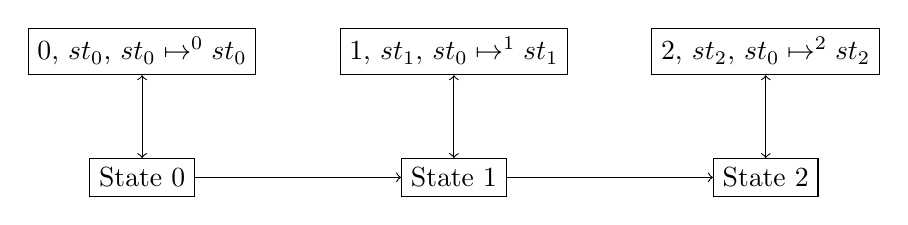
\begin{tikzpicture}[node distance=10pt]
    \node[draw] (Description 0)  {0, $st_{0}$, $st_{0}\mapsto^{0}st_{0}$};
    \node[draw, right=30pt of Description 0] (Description 1)  {1, $st_{1}$, $st_{0}\mapsto^{1}st_{1}$};
    \node[draw, right=30pt of Description 1] (Description 2)  {2, $st_{2}$, $st_{0}\mapsto^{2}st_{2}$};
    
    \node[draw, below=30pt of Description 0]    (State 0)  {State 0};
    \node[draw, below=30pt of Description 1]    (State 1)  {State 1};
    \node[draw, below=30pt of Description 2]    (State 2)  {State 2};
    

    \graph{
        (State 0) -> (State 1) -> (State 2);
        (State 0) <-> (Description 0);
        (State 1) <-> (Description 1);
        (State 2) <-> (Description 2);
    };
\end{tikzpicture}

Then, we construct a bijection relation between reachable state set and Fin N.
\begin{code}%
    \AgdaBound{St-Fin} %
    \AgdaSymbol{:} %
    \AgdaFunction{∃[} %
    \AgdaBound{m} %
    \AgdaFunction{]} %
    \AgdaFunction{∃[} %
    \AgdaBound{stₘ} %
    \AgdaFunction{]} %
    \AgdaSymbol{(}\AgdaBound{st₀} %
    \AgdaOperator{\AgdaDatatype{↦[}} %
    \AgdaBound{m} %
    \AgdaOperator{\AgdaDatatype{]}} %
    \AgdaBound{stₘ}\AgdaSymbol{)} %
    \AgdaOperator{\AgdaFunction{⤖}} %
    \AgdaDatatype{Fin} %
    \AgdaBound{N}\<%
    \\
\end{code}

It seems like all reachable states are indexed by one of element in Fin N set.
\vspace{1em}

\usetikzlibrary{graphs, positioning, quotes, shapes.geometric}

\begin{document}
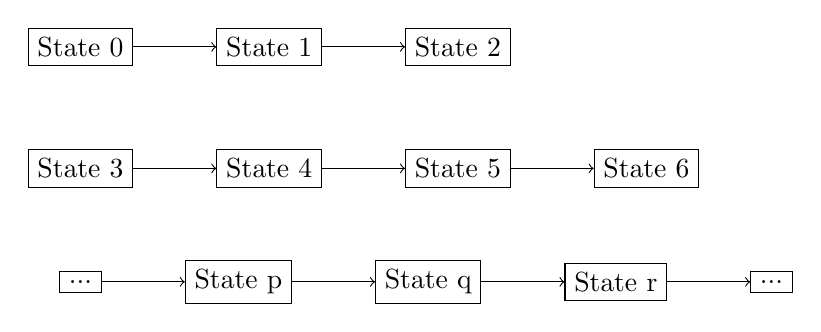
\begin{tikzpicture}[node distance=10pt]
    \node[draw]                           (State 0)  {State 0};
    \node[draw, right=30pt of State 0]    (State 1)  {State 1};
    \node[draw, right=30pt of State 1]    (State 2)  {State 2};
    
    \node[draw, below=30pt of State 0]    (State 3)  {State 3};
    \node[draw, right=30pt of State 3]    (State 4)  {State 4};
    \node[draw, right=30pt of State 4]    (State 5)  {State 5};
    \node[draw, right=30pt of State 5]    (State 6)  {State 6};


    \node[draw, below=30pt of State 3]    (another)  {...};
    \node[draw, right=30pt of another]    (State p)  {State p};
    \node[draw, right=30pt of State p]    (State q)  {State q};
    \node[draw, right=30pt of State q]    (State r)  {State r};
    \node[draw, right=30pt of State r]    (others)  {...};

    \graph{
        (State 0) -> (State 1) -> (State 2);
        (State 3) -> (State 4) -> (State 5) -> (State 6);
        (another) -> (State p) -> (State q) -> (State r) -> (others);
    };
\end{tikzpicture}

Combine the definition above, and we have the exact definition of Broad RevTerminate Principle:
\begin{code}%
    \>[2]\AgdaFunction{Finite-Reachable-State-Termination} %
    \AgdaSymbol{:} %
    \AgdaSymbol{∀} %
    \AgdaSymbol{\{}\AgdaBound{N} %
    \AgdaBound{st₀}\AgdaSymbol{\}}\<%
    \\
    \>[2][@{}l@{\AgdaIndent{0}}]%
    \>[4]\AgdaSymbol{→} %
    \AgdaSymbol{(}\AgdaBound{St-Fin} %
    \AgdaSymbol{:} %
    \AgdaFunction{∃[} %
    \AgdaBound{m} %
    \AgdaFunction{]} %
    \AgdaFunction{∃[} %
    \AgdaBound{stₘ} %
    \AgdaFunction{]} %
    \AgdaSymbol{(}\AgdaBound{st₀} %
    \AgdaOperator{\AgdaDatatype{↦[}} %
    \AgdaBound{m} %
    \AgdaOperator{\AgdaDatatype{]}} %
    \AgdaBound{stₘ}\AgdaSymbol{)} %
    \AgdaOperator{\AgdaFunction{⤖}} %
    \AgdaDatatype{Fin} %
    \AgdaBound{N}\AgdaSymbol{)}\<%
    \\
    %
    \>[4]\AgdaSymbol{→} %
    \AgdaSymbol{(}\AgdaBound{has-next} %
    \AgdaSymbol{:} %
    \AgdaSymbol{∀} %
    \AgdaSymbol{(}\AgdaBound{st} %
    \AgdaSymbol{:} %
    \AgdaField{State}\AgdaSymbol{)} %
    \AgdaSymbol{→} %
    \AgdaRecord{Dec} %
    \AgdaSymbol{(}\AgdaFunction{∃[} %
    \AgdaBound{st'} %
    \AgdaFunction{]} %
    \AgdaSymbol{(}\AgdaBound{st} %
    \AgdaOperator{\AgdaField{↦}} %
    \AgdaBound{st'}\AgdaSymbol{)))}\<%
    \\
    %
    \>[4]\AgdaSymbol{→} %
    \AgdaFunction{is-initial} %
    \AgdaBound{st₀}\<%
    \\
    %
    \>[4]\AgdaSymbol{→} %
    \AgdaFunction{∃[} %
    \AgdaBound{stₙ} %
    \AgdaFunction{]} %
    \AgdaSymbol{(}\AgdaBound{st₀} %
    \AgdaOperator{\AgdaDatatype{↦*}} %
    \AgdaBound{stₙ} %
    \AgdaOperator{\AgdaFunction{×}} %
    \AgdaFunction{is-stuck} %
    \AgdaBound{stₙ}\AgdaSymbol{)}\<%
    \\
\end{code}
